\documentclass[12pt, a4paper]{article}
    \usepackage[utf8]{inputenc}
    \usepackage[czech]{babel}
    \usepackage{amsmath, amsthm, amssymb}
    \usepackage{mathtools}
    \usepackage{graphicx}
    \usepackage{tabularx}
    \usepackage{enumitem}
    \usepackage{tabto}
    \pagestyle{empty}

    \setlength{\oddsidemargin}{-15pt} %-72
    \setlength{\textwidth}{494pt} %598
    \setlength{\voffset}{-60pt} %-50
    \setlength{\headheight}{0pt}
    \setlength{\textheight}{710pt}
    \TabPositions{-5pt}

    \graphicspath{{C:\Users\Bohdan\Documents\School\Physics\kapilarni_jevy}}
    \addto\captionsczech{\renewcommand{\figurename}{Obrázek č.}}

\begin{document}
% HLAVIČKA
\hfill Bohdan Kopčák a Markéta Sázavská\par
\hfill Sexta B\par
\hfill {\it Protokol vypracován dne 20. 6. 2018}\par

\section*{\indent 4. laboratorní práce}
% ŘEŠENÍ
\tab \textbf{Téma: }
Kapilární elevace\\[4pt]
\tab \textbf{Úkol: }
Změřte, do jaké výšky vystoupá voda při kapilární elevaci a vypočtěte povrchové napětí vody.\\[4pt]
\tab \textbf{Pomůcky: }
kapilára, kádinky, milimetrové měřítko, mikrometr, jehla, voda\\[4pt]
\tab \textbf{Teorie: }
Povrchovou sílu $F_p$ lze vypočítat vztahem $F_p = \sigma \cdot l$ z čehož lze odvodit, že 
$$\sigma = \dfrac{F_p}{l}$$
kde $F_p$ je povrchová síla a $l$ je délka okraje povrchové vrstvy.

% OBRÁZEK
\begin{minipage}{0.4\textwidth}
    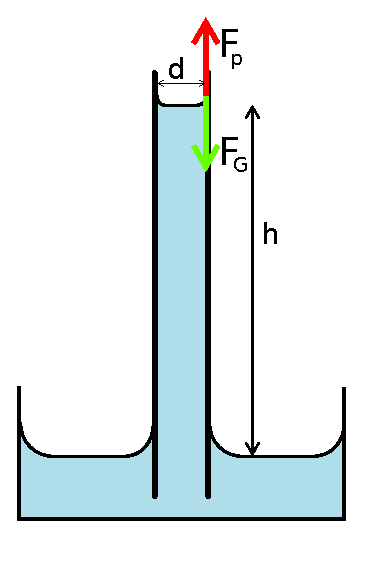
\includegraphics[width = 1\textwidth]{kapilara.eps}
\end{minipage}
% SIDE TEXT
\begin{minipage}{0.6\textwidth}
    \tab \textbf{nahoru }
    působí reakce k povrchové síle ($F_p = F$)
    $$F = \sigma \cdot l = \sigma \cdot 2\pi r = \sigma \cdot \pi d$$
    \tab \textbf{dolů }
    působí tíhová síla $F_G$
    $$F_G = \rho \cdot V \cdot g = \rho \cdot \pi \dfrac{d^2}{4} \cdot h \cdot g$$

    $$F = F_G$$
    $$\sigma \cdot \pi \cdot d = \rho \cdot \pi \cdot d^2 \cdot 4^{-1} \cdot h \cdot g$$
    $$\sigma = \rho \cdot d \cdot h \cdot g \cdot 4^{-1}$$
    $$\sigma = \dfrac{\rho \cdot d \cdot h \cdot g}{4}$$
\end{minipage} \par

\tab \textbf{Postup: }
\begin{enumerate}
    \item Zasuneme do kapiláry jehlu a pomocí její tloušťky v bodě kde se zasekne určíme tloušťku vnitřní části kapiláry.
    \item Kapiláru ponoříme do kádinky a smočíme její stěny.
    \item Kapiláru vytáhneme tak, aby byl dolní konec těsně pod hladinou vody.
    \item Naměříme výšku hladiny v kapiláře.
    \item Kroky 2. až 4. opakujeme až do získání patřičného počtu měření.
\end{enumerate} \par
\pagebreak
\tab \textbf{Teorie výpočtu odchylky:}\\
{
    \hspace{1.4em}
    $d$ je naměřená hodnota\\
    $\overline{d}$ je aritmetický průměr $d$\\
    $\Delta d$ je absolutní chyba, což je odchylka daného měření od $\overline{d}$\\
    $\delta d$ je relativní chyba($\dfrac{\Delta d}{\overline{d}}$)
} 

% TABULKA
\tab \textbf{Naměřené hodnoty a výsledky měření:}\footnote{Průměrné hodnoty jsou již zaokrouhleny na platný počet desetinných míst.}\\[6pt]
\begin{tabular}{r|c c|c c}
    {č. měření} & {$d$[mm]} & {$\Delta d$[mm]} & {$h$[mm]} & {$\Delta h$[mm]}\\
    \hline
    1 & 0,75 & 0,01 & 37 & 0\\
    2 & 0,75 & 0,01 & 36 & 1\\
    3 & 0,72 & 0,02 & 38 & 1\\
    \hline
    {průměr} & 0,740 & 0,01 & 37,0 & 1
\end{tabular}\\[20pt]

\begin{align*}
    \mathllap{d} &= (0,74 \pm 0,01)\cdot 10^{-3} m, \delta d = 1,4\% \\
    \mathllap{h} &= (37 \pm 1)\cdot 10{^-}3 m, \delta h = 2,7\% \\
    \vspace{5em}
    \phantom{\delta \sigma}
    \phantom{\Delta \sigma}
    \mathllap{\sigma} &= \dfrac{\rho \cdot d \cdot h \cdot g}{4} \\
    \mathllap{\sigma} &= \dfrac{\rho = 998 kg \cdot m^{-3} \cdot 0,74 \cdot 10^{-3} m \cdot 37\cdot 10^{-3} m \cdot 9,81 m \cdot s^{-2}}{4} \\
    \mathllap{\sigma} &= 67 \cdot 10^{-3} N \cdot m^{-1} \\
    \vspace{2em}
    \mathllap{\delta \sigma} &= \delta \rho + \delta d + \delta h + \delta g = 0\% + 1,4\% + 2,7\% + 0\% \\
    \mathllap{\delta \sigma} &\doteq 4,1\% \\
    \vspace{2em}
    \mathllap{\Delta \sigma} &= \dfrac{\sigma}{100} \cdot \delta \sigma = \dfrac{67 \cdot 10^{-3} N \cdot m^{-1}}{100} \cdot 4,1\% \\
    \mathllap{\Delta \sigma} &\doteq 3 \cdot 10^{-3} N \cdot m^{-1}
\end{align*}\\[10pt]
\tab \textbf{Závěr: }
Hodnota $\sigma$, kterou jsme naměřili, byla $(67 \pm 3) \cdot 10^{-3} N \cdot m^{-1}$.
Tato hodnota je nižší, než hodnota tabulková $(73 \cdot 10^{-3} N \cdot m^{-1})$, což je zaviněno především znečištěním vody.\\[4pt]
Sazba byla provedena programem \LaTeX
\end{document}